\documentclass{article}
\usepackage[utf8]{inputenc}
\usepackage{amsmath}
\usepackage{amsthm}
\usepackage{amssymb}
\newtheorem{theorem}{Theorem}[section]
\newtheorem{corollary}{Corollary}[theorem]
\newtheorem{lemma}[theorem]{Lemma}

\usepackage[colorlinks=true]{hyperref}
\usepackage[linesnumbered,algoruled,boxed,lined]{algorithm2e}
\usepackage{graphicx}
\usepackage{caption}
\usepackage{float}
\usepackage{multirow}
\usepackage{placeins}
\usepackage{hhline}

\def\d{\,{\rm d}}               % differential
\def\vc#1{\mathbf{\boldsymbol{#1}}}     % vector
\def\tn#1{\mathbb{#1}}
\def\eps{\varepsilon}
\def \E{{{\rm I\kern-.3em E}}}
\def \D{{{\rm I\kern-.3em D}}}
\newcommand{\norm}[1]{\left\lVert#1\right\rVert}
\def\prtl{\partial}
\def\todo#1{{\color{red}TODO: #1}}
\def\R{\mathbf{R}}
\def\pluseq{\mathrel{+}=}

\def\Bavg#1{\Left\langle#1\Right\rangle}
\def\avg#1{\langle#1\rangle}
\def\Var{\mathop{\rm Var}}
\def\abs#1{|#1|}
\DeclareMathOperator{\Span}{span}

\title{Application of Multilevel Monte Carlo Maximum Entropy method to Contaminant Transport}
\author{jan.brezina }
\date{September 2018}


\begin{document}

\maketitle

\section{Introduction}
Long term safety of an underground radioactive waste repository is assured primarily by the dilution and 
very slow transport of the contaminants through the suitable rock formations. Maximal concentrations of the contaminant on the surface is of major concern. Unfortunately reliable prediction of the surface concentration is not tractable due to lack of data about highly heterogeneous rock environment. In order to deal with these uncertainties we can model unknown rock properties as random fields and predict probability density function of the surface density. 
Classical Monte Carlo method needs at least several thousands of samples, which is prohibitively costly in the case of complex simulations. The Multilevel Monte Carlo (MLMC) method introduced by Giles \cite{Giles2008}, \cite{Giles2015} provides a way to estimate mean of an observable at the cost comparable to few forward simulations. Basic idea is to do high volume of samples using a less accurate but cheap approximation and much fewer samples of the difference between the observable and its approximation. If the difference have much smaller variance we obtain the mean estimate with same accuracy at fraction of cost.  The MLMC method has been already studied and analyzed in connection with variety of PDE problems: elliptic equations \cite{Barth2011a}, \cite{Cliffe2011a}, \cite{Abdulle2013}, parabolic equations \cite{Barth2013},
multiphase flow \cite{Muller2013}, \cite{Lu2016} and other.


Maximal entropy:
\cite{Barron1991}, \cite{Bierig2016a}

Elliptic eq. with log normal coefficients \cite{Graham2015}






 However the limitation is that MLMC can compute only approximation of expectation of any random variable. Therefore it is straight forward to make approximation of the mean, the variance and other moments, while it is not possible to approximate the quantiles and the distribution function directly. On the other way, the moment function or characteristic function are given in terms of expectations, which motivates a general approximation of the density function in terms of generalized moments.

Possible outcomes:
\begin{itemize}
    \item Research for suitable statistical models for complex hydrology problems (porosity, conductivity, dispersion, fracture openning, fracture density, ... dependency on the length scale).
    \item Demonstrate efficiency of MLMC for estimation various moments of relevant quantities of interest.
    \item Demonstrate efficient generation of samples for various types of correlations.
    \item Demonstrate reconstruction of the density function.
\end{itemize}

\section{Multilevel Monte Carlo method}
In this section we shall introduce the MLMC estimator and consider its application to a random variable based on a solution to a PDE.
Let $(\Omega, \Sigma, P)$ be a probability space and $X(\omega)$ be a random variable
which can not be sampled exactly, but we are able to sample its approximation $X^h(\omega)$. 
Consider classical MC approximation of the mean value $\E X$ by the sample mean:
\[
	\avg{X^h}_N = \frac{1}{N}\sum_{i=1}^{N} X^h(\omega_i).
\]
Mean square error or variance of this estimator can be decomposed as:
\[
	\Var[ \avg{X^h}_N - \E X ] = \frac{1}{N} \Var X^h + \abs{\E X^h - \E X}^2
\]
where the first part is the sampling error and the second part is error of the approximation $X^h$. Classical MC method diminish the sampling error just by increasing $N$. The idea of MLMC method is to introduce another approximation $X^H$ that is cheaper to sample and use the composed estimator
\[
	\E X^h \approx \avg{X^h}_{M,N} = \avg{X^H}_M	 + \avg{X^h - X^H}_N, 
\]
with variance
\[
	\Var[\avg{X^h}_{M,N} - X^h] =  \frac{1}{M}\Var{X^H} + \frac{1}{N}\Var[X^h-X^H]. 
\]
Now we can increase precision of the estimator by increasing the number $M$ of the cheap coarse samples, while keeping the number $N$ of the expensive fine samples low provided the variance of
$\Var[X^h-X^H]$ is small.

Using a sequence of approximations $X^l = X^{h_l}$, for $l=1,\dots, L$ and $X^0 = 0$, we obtain the MLMC estimator:
\begin{equation}
    \label{eq:mlmc_est}
	\E X^L \approx \avg{X^L}_{\vc N} = \sum_{l=1}^L \avg{X^l - X^{l-1}}_{N_l} 	= \sum_{l=1}^L \avg{\Delta X^l}_{N_l}
\end{equation}
where $\vc N=(n_1,\dots, n_L)$ is the \emph{sampling vector} and $\Delta X^l(\omega) =X^l(\omega) - X^{l-1}(\omega)$. Variance of the MLMC estimator is:
\begin{equation}
    \label{eq:var_mlmc}
	\Var \avg{X^L}_{\vc N} = \sum_{l=1}^L \frac{V_l}{N_l},\quad V_l = \Var \avg{\Delta X^l}_{N_l}.
\end{equation}

In particular we are interested in the case $X=F(u)$, where $F$ is a functional representing an observation of
the solution $u$ to a PDE with random data $d(\omega)$. The approximations $X^l = F(u^{h_l})$ are same observations
for an approximate solution $u^{h_l}$ computed using a mesh with step $h_l$. Let $u$ be from a space $W$, $u_h$ from $W_{h_l} \subset W$ and assume a usual error estimate in the form:
\[
	\norm{u - u_h}_{W} \le h^s \norm{u}_{W^*}.
\] If $F:W \to R$ is bounded, then for $h=h^l$, $H=h^{l-1}$, we have
\[
	\abs{X^l - X^{l-1}} = \abs{F(u^h) - F(u^H)} \le \norm{F}\norm{u^h - u^H}_W \le C H^s\norm{u}_{W^*}
\]
and therefore 
\begin{equation}
    \label{eq:level_var_pde_est}
    V_l =  \mathcal O( h_{l-1}^{2s}).
\end{equation}
By the same token we have 
\begin{equation}
    \label{eq:aprox_pde_est}
    \abs{\E X - \E X^L)}^2 = \mathcal O( h_L^{2s} ).
\end{equation}
\todo{Vhodna literatura, kde je toto udelano poradne alespon pro ellipticky pripad.}
The cost $C_l$ of evaluation of the single sample $X^{l-1}(\omega) - X^l(\omega)$ is $C_l \approx  h_l^{-\gamma}$, e.g. an efficient solver of an elliptic equation have $\gamma=d$  where $d=1,2,3$ is the dimension of the problem. 

\subsection{Optimal choice of number of samples}
Efficiency of the MLMC estimator \eqref{eq:mlmc_est} depends on the optimal choice of the sample vector $\vc N$. Let  the level variances $V_l$ be given and let us denote $C_l$ the computational cost of a single sample of the difference $\Delta X^l$ at the level $l=1,\dots, L$. For a given target variance $V$ (c.f. \eqref{eq:var_mlmc}), we want to minimize the total cost
\begin{equation}
    \label{eq:total_cost}
	C = \sum_l C_l N_l.
\end{equation}
This leads to minimization problem for the functional
\[
	\Phi(N_1, \dots, N_L,\lambda) = \sum_l C_l N_l + \lambda \Big(\sum_l \frac{V_l}{N_l} - V\Big).
\]
Straightforward calculation then provides optimal choice of $\vc N$ for given $V$ reported already in \cite{Giles2015}:
\begin{equation}
	\label{opt_n_for_var}
	N_l^V = \sqrt{\frac{V_l}{C_l}} \frac{\sum_i \sqrt{V_i C_i}}{V}, \quad \text{for }l=1,\dots, L.
\end{equation}
Similarly we obtain $\vc N$ that minimize the total variance for the fixed total cost $C$ as
\begin{equation}
	\label{opt_n_for_cost}
	N_l^C = \sqrt{\frac{V_l}{C_l}} \frac{C}{\sum_i \sqrt{V_i C_i}}
	, \quad \text{for }l=1,\dots, L.
\end{equation}

Formulas \eqref{opt_n_for_var} and \eqref{opt_n_for_cost} are based on the knowledge of the level variances $V_l$ and computational costs $C_l$ which are usually not known and must be estimated (see Section \ref{sec:VarEst}). These small errors lead to large changes in the optimal sample vector since related minimized functionals are quite flat at the optimal point.  This often results in overestimating the number of samples, especially on lower levels. To mitigate this problem we rather use
\[
	N_l^{V*} = \min( N_l^V, \frac{V_l L}{V} )
\]
for prescribed total variance $V$ and
\[
	N_l^{C*} = \min( N_l^C, \frac{C}{C_l L} )
\]
in the case of fixed cost $C$. This modification increase the total variance or total cost at most by $V$ and $C$ respectively, while keeping  $N_l$ reasonable. Indeed, let
\[
	N_l^{V*} = \frac{V_l L}{V} < N_l^V 
\]
happen for a single level $l$, then increase in the total variance is
\[
    V^* - V = \frac{V}{L} - \frac{V_l}{N_l^V} \le \frac{V}{L}
\]
and similarly for $N_l^{C*}$.



\subsection{Estimate level variance}
\label{sec:VarEst}
In order to make MLMC algorithm fully automatic we want to estimate level variances $V_l$ from already collected samples. Since direct estimates are too inaccurate for higher levels we rather setup a regression model for $V_l$ and estimate its parameters using data 
from all levels. Moreover we also combine data for different moments.

Let us assume that the level difference $Z_l^r = X_l^r - X^r_{l-l}$ for level $l=1,\dots L$ and a moment $r$ is normally distributed 
with mean estimate $\hat{Z}_l^r$ and variance estimate $V_l^r$ is
$$
W_l^r = \sum_{i} (Z^r_{l,i} - \hat{Z}_l^r)^2 / (n_l - 1).
$$

Where $Y_l = (n_l -1)W_l^r/V_l^r$ have distribution $\chi^2_{n_l -1}$.

We assume a simple model:
$$
  U_l^r = \log W_l^r =  \alpha_r + \beta \log h_l + \gamma (\log h_l)^2.
$$
where $h_l$ is a mesh step on level $l$ and $\alpha_r$, $\beta$ are parameters. 
For the variance of $U_l^r$ we have:
$$
  \D U_l^r = \D \log \Big( \frac{Y_l V_l^r}{n_l - 1} \Big) = \D \log (Y_l/N_l) = \epsilon_l
$$
with $N_l = n_l - 1$.

Then we estimate model parameters $\alpha_r$, $\beta$ from the least squares problem:
$$
    \tn{X}^T \tn{D}^2 \tn{X} \vc{b} = \tn{X}^T \tn{D} \vc{U},
    \ D_{i,i} = 1/\epsilon_{l}.
$$

Values of $\epsilon_l$ as a function of $l$ will be determined by MC. Note also that using the \href{https://en.wikipedia.org/wiki/Probability_density_function#Dependent_variables_and_change_of_variables}{Jacobi transform} we obtain PDF of $\epsilon_l$ as:
$$
    f(\epsilon) = \exp(\epsilon)N_l\chi^2_{n-1}(\exp(\epsilon)N_l).
$$
For small values of $N_l$ we compute $\D \epsilon_l$ using numerical quadrature. For sufficiently large $N_l$ we approximate $\chi^2$ by normal distribution:
$$
    f(\epsilon) = \exp(\epsilon)N_l\chi^2_{n-1}(\exp(\epsilon)N_l).
$$
\subsubsection{Uvahy}
Cilem je ziskat odhad rozptylu MLMC estimatoru, tak aby skutecny rozptyl byl mensi s danou pravdepodobnosti. 

Notes:
\begin{itemize}
    \item Variance $W_l$ of the level variance estimator is:
    \[
        Var \hat\sigma_l^2 \approx \hat\sigma_l^2 \frac{2}{N_l - 1}
    \]
    \dots assuming
    \[
    Z_l = \sum_{i=1}^{n_l}\Big(\frac{\Delta X^l_i}{\sigma_l}\Big)^2
    \]
    be approximately $\chi^2_k$ with $k=n_l$. This corresponds to the assumption that level differences $\Delta X_l$ have normal distribution. 
    \item At least for flow test case it seems that higher moments have smaller $W_l$ then first few (up to 10) moments. The differences in $W_l$ for individual moments are about one order of magnitude.  This effect is more pronounced for levels with many samples so it seems to be real. Differences between levels are also about one order of magnitude.
    \item These observations are not in contradiction with approximation of variance of  $\log W_l$.
\end{itemize}




\subsection{MLMC sampling algorithm}
Optimal choice of the sample vector $\vc N$ given by \eqref{opt_n_for_var} or \eqref{opt_n_for_cost} is function $N^{opt}(\vc V, \vc C)$ of the vector of level variances $\vc V$ and the vector of level costs $\vc C$. As $\vc V$ and $\vc C$ are not known a priori, we want to estimate them on the fly from the increasing set of collected samples. as we collect the samples.  Level variances $V_l$ are estimated by the regression \eqref{eq:regression}, sample cost $C_l$ is simply the average sample time of collected samples on the level $l$. 
In order to collect optimal number of samples we designed a simple iterative Algorithm \ref{algo_sampling}. 
Initial vector of scheduled samples $N^s_0$ is fixed, in particular we use an arithmetic sequence decreasing form $100$ to $0$. Vector $\vc N^t_0$ of target number of samples is set to $2\,\vc N^s_0$. The iteration $i$ starts with scheduling new samples up to the $\vc N^s_i$.
Then we wait until at least half of $N^s_i$ is computed. \todo{"half of samples is done" ... to je divne, neni jasne pulka kterych by to mela byt, a jestli to musi byt pulka.}. We collect computed samples and use all available samples to update estimates $\vc V_i$ and $\vc C_i$ for level variances and costs respectively.
Using these new estimates we determine new target sampling vector $\vc N^t_{i+1}$ and
add fraction $\alpha$ of the difference to $\vc N^t_{i}$. We iterate until relative difference between target and scheduled sampling vectors is greater then tolerance $\epsilon$ for any level $l$.
In practice we use parameters $\alpha=0.1$ and $\epsilon = 0.0$

\begin{algorithm}
    \SetAlgoLined
    \DontPrintSemicolon
    %
    $\vc N^s_0 \gets ( 100, ..., 3)$\;
    $\vc N^t_0 = 2 \vc N^s_0$\;
    $i \gets 0$\;
    \While{ $N^t_{i,l} - N^s_{i,l} > \eps N^s_{i,l}$ for any $l$ }{
        schedule new samples up to $\vc N^s_i$\;
        wait until half of samples is done\;
        estimate $\vc V_i$, $\vc C_i$ from collected samples\;
        $\vc N^t_{i+1} \gets N^{opt}(\vc V_i, \vc C_i)$\;
        $\vc N^s_{i+1} \gets \vc N^s_i + \alpha(\vc N^t_{i+1} - \vc N^s_i)$\;
        $i \gets i+1$\;
    }
    \label{algo_sampling}
    \caption{MLMC samples number estimation}
\end{algorithm}

Progress of the algorithm is depicted at Figure \ref{fig:n_l_time}.  ... 

\break
Following graph \ref{fig:n_l_time} and table \ref{mlmc_sampling} provide data for the task of water flowing through unit square using flow123d \cite{flow123d} software. We use five level MC method. Different meshes were created at different levels. First level mesh had just 6 elements, higher levels had meshes with 78, 1730, 40818 and 997606 elements. Whole task was performed on cluster that contains 20 nodes each of them has 2x 10-core CPU and 96 GB RAM, this allowed us to perform parallel computing of samples. Individual sample computations were grouped to the jobs that were scheduled in cluster by PBS software. Each job had approximately same computational cost. Cluster traffic affects the number of currently running jobs. As a result, it can affect the fluency of the sample computations. That probably caused jump $C^c$ around 40th iteration in \ref{fig:n_l_time}.

\todo{Popsat jake byly velikosti siti na jednotlivych urovnich a jaka to vubec byla uloha. Popsat zhruba HW na kterem to bezelo, a davkove zpracovani pomoci PBS. Okomentovat nerovnomerny prubeh krivky dokoncenych vzorku.}
\begin{figure}[H]
\centering
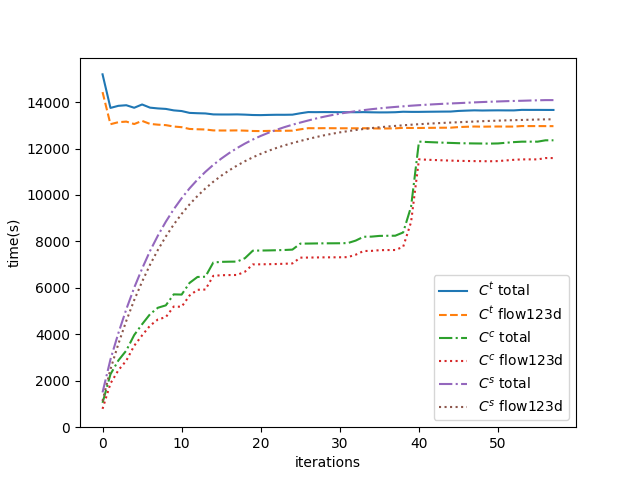
\includegraphics[width=\textwidth]{time_1.png}
\label{fig:n_l_time}
\caption{Evolution of CPU time for target $C^t$, scheduled $C^s$ and collected samples during iterations of Algorithm \ref{algo_sampling}.}
\end{figure}
\todo{Upravit typ car: barvou rozlisit $C^s$, $C^t$, $C^c$, plnou carou kompletni cas, carkovane pouze vypocet Flow123d. Tu carkovanou bych udelal jen pro $N_c$. Takze by tam nakonec byly 4 cary.}
V tomto grafu jsou $C^s$ - naplánované vzorky (estimated), $C^c$ jsou již dokončené vzorky (collected), $C^t$ jsou cílové vzorky pokud bychom je určovali z $C^c$. Po skončení celé MLMC by byly $C^c$ a $C^s$ stejné, $C^t$ jsou na konci menší než $C^s$, protože se ukazuje, že jsme na začátku napočítali více vzorků na nižších úrovních [17, 7, 3] a stačilo by [12, 2, 2]. Různý typ čar jsem zvolil kvůli tomu kdyby to nakonec bylo černobíle, tak aby to bylo k přečtení. Pokud by tam zůstali ty přidané křivky, tak už by to nešlo oddělit stylem čáry. 
\todo{Proc je graf nakonci uriznuty? Mozna tu tabulku uplne zrusime, ale do grafu by se tedy jeste hodil odhadovany cas naplanovanych uloh. To je asi ten cas estimated v tabulce.  Bylo by z toho snad videt, ze mame celou dobu previs naplanovanych uloh na provedenymi.}

\begin{table}[]
\caption{Sampling algorithm iterations}
\centering

\begin{tabular}{|l|l|l|l|l|l|l|}
\hline
iteration                                  & samples  & $l_{1}$     & $l_{2}$   & $l_{3}$  & $l_{4}$ & $l_{5}$ \\ \hhline{|=|=|=|=|=|=|=|}
{\multirow{2}{*}{0}} & collected & 100    & 41    & 17  & 7  & 2  \\ 
                   & estimated & 2204   & 402   & 17  & 7  & 3  \\ \hline
\multirow{2}{*}{1}                       & collected & 1112   & 402   & 17  & 7  & 3  \\  
                                         & estimated & 3955   & 612   & 17  & 7  & 3  \\ \hline
\multirow{2}{*}{2}                       & collected & 2103   & 432   & 17  & 7  & 3  \\  
                                         & estimated & 5545   & 801   & 17  & 7  & 3  \\ \hline
% \multirow{2}{*}{3}                       & collected & 2789   & 481   & 17  & 7  & 3  \\  
%                                          & estimated & 6982   & 971   & 17  & 7  & 3  \\ \hline
\multirow{2}{*}{4}                       & collected & 3777   & 654   & 17  & 7  & 3  \\  
                                         & estimated & 8261   & 1118  & 17  & 7  & 3  \\ \hline
% \multirow{2}{*}{5}                       & collected & 4455   & 785   & 17  & 7  & 3  \\ 
%                                          & estimated & 9435   & 1253  & 17  & 7  & 3  \\ \hline
\multirow{2}{*}{10}                      & collected & 6517   & 926   & 17  & 7  & 3  \\  
                                         & estimated & 12979  & 1642  & 17  & 7  & 3  \\ \hline
% \multirow{2}{*}{15}                      & collected & 8668   & 1216  & 17  & 7  & 3  \\  
%                                          & estimated & 15646  & 1920  & 17  & 7  & 3  \\ \hline
\multirow{2}{*}{20}                      & collected & 9457   & 1268  & 17  & 7  & 3  \\  
                                         & estimated & 17181  & 2078  & 17  & 7  & 3  \\ \hline
% \multirow{2}{*}{25}                      & collected & 9950   & 1287  & 17  & 7  & 3  \\ 
%                                          & estimated & 18081  & 2172  & 17  & 7  & 3  \\ \hline
\multirow{2}{*}{30}                      & collected & 9972   & 1293  & 17  & 7  & 3  \\  
                                         & estimated & 18671  & 2247  & 17  & 7  & 3  \\ \hline
% \multirow{2}{*}{35}                      & collected & 10488  & 1322  & 17  & 7  & 3  \\ \ 
%                                          & estimated & 19021  & 2292  & 17  & 7  & 3  \\ \hline
% \multirow{2}{*}{40}                      & collected & 16739  & 2102  & 17  & 7  & 3  \\  
%                                          & estimated & 19233  & 2317  & 17  & 7  & 3  \\ \hline
% \multirow{2}{*}{45}                      & collected & 16656  & 2065  & 17  & 7  & 3  \\  
%                                          & estimated & 19368  & 2334  & 17  & 7  & 3  \\ \hline
% \multirow{2}{*}{50}                      & collected & 16647  & 2055  & 17  & 7  & 3  \\  
%                                          & estimated & 19473  & 2355  & 17  & 7  & 3  \\ \hline
% \multirow{2}{*}{54}                      & collected & 16747  & 2050  & 17  & 7  & 3  \\  
%                                          & estimated & 19504  & 2361  & 17  & 7  & 3  \\ \hline
\multirow{2}{*}{55}                      & collected & 16782  & 2051  & 17  & 7  & 3  \\  
                                         & estimated & 19544  & 2370  & 17  & 7  & 3  \\ \hline
\multirow{2}{*}{56}                      & collected & 16783  & 2051  & 17  & 7 & 3  \\  
                                         & estimated & 19556  & 2373  & 17  & 7 & 3  \\ \hline
\end{tabular}
\end{table}
\FloatBarrier



\section{Maximal Entropy method}
The MLMC  estimator \eqref{eq:mlmc_est} can reuse the set of collected samples $X^l_i$ to estimate also any generalized moment of the random variable $X$. In this section we will use a finite set of moments to construct an approximation to the density function of $X$.

Let $X$ be a continuous random variable with density function $\rho$
and assume then $supp(\rho) \subset \Omega$ for a bounded.
interval $\Omega \subset \R$. Further consider generalized moments
\begin{equation}
    \label{eq:gen_moments}
    \mu_r = \E_{\rho}[\phi_r(X)], \quad 
\end{equation}
for a finite set of linearly independent moment functions $\phi_r\in L^2(\Omega, \rho)\cap L^1(\Omega, \rho)$, $r=1,\dots, R$ generating the space
\[
    \mathcal V = \Span\{\phi_r, r=1,\dots, R\}.
\] We shall use also the vector notation $\vc \phi = (\phi_1, \dots,\phi_R)$. \todo{Define spaces $L^p(\Omega, \rho)$.}

The same set of collected samples $X^l_i$ can be reused to compute MLMC estimates of  moments $\mu_r$ as
\[
	\hat\mu_r = \sum_{l=1}^L \avg{\phi_r(X^l) - \phi_r(X^{l-1})}_{N_l}.
\]

Now we want to find an approximation $\rho^R$ to the unknown density $\rho$ using only the exact moments $\vc \mu$. There is infinite many of such densities so we choose the one that maximize Shanon's entropy:
\[
    S(\rho) = - \E_\rho \log \rho
\], which corresponds to the minimization of any additional information. 
In more general setting we may assume a density $p$ of a prior distribution. And minimize the Kullbeck-Leibler divergence:
\[
    D(\rho||p) = \int \rho(x) \ln(\rho(x)/ p(x) \d x.
\]
This leads to the minimization of the functional:
\begin{align}
    \Phi(\rho, \vc\lambda) 
    &= 
    \int \rho \Big( \vc\lambda \cdot \vc \phi - \log(\rho/p) \Big) \d x - \vc\lambda \cdot \vc\mu.
\end{align}
Setting the variation with respect to $\rho$ equal to zero leads to
the approximation in the from:
\[
    \rho^R(x) = p \exp\Big\{\vc \lambda \cdot \vc \phi \Big\}
\]
if we assume $\phi_0(x) = 1$. The parameter$\vc\lambda$ is solution
to the nonlinear system of equations:
\begin{equation}
    \label{eq:moment_system}
    \int \vc\phi\, p e^{\vc\lambda\cdot \vc\phi}\d x = \vc \mu
\end{equation}
with the Jacobi matrix:
\[
    \tn H = \int \vc\phi \otimes \vc \phi\, 
    p e^{\vc\lambda\cdot\vc\phi} \d x.
\]

\begin{lemma}
If $p$ is strictly positive and measurable on $K_n$ and functions $\phi_r$ are linearly independent, then matrix $\tn H$ is symmetric positive definite for any $\vc \lambda$.
\end{lemma}
First assume that functions $\phi_r(x)$ form an ortonormal set with respect to the space $L^2(K_n)$. Then for any non-zero $\vc u$ from $\R^R$  we have:
\[
    \vc u^T \tn H \vc u = \int_{K_n} \Big\{\sum_r u_r \phi_r(x)\Big\}^2 p(x) \exp\Big\{ \vc\lambda\cdot \vc\phi(x)\Big\} \d x \ge k \norm{U}^2_{L^2(K_n)} > 0
\]
for some $0< k \le p(x)\exp\Big\{ \vc\lambda\cdot \vc\phi(x)\Big\}$.

\subsection{Projection to exponential family}
Further on all densities are considered on $\Omega$.
Following \cite{Barron1991}, for a given $\vc \mu$ let us define
set of densities with appropriate moments:
\[
    C_{\vc \mu} = \{ \rho : \E_\rho[\vc \phi] = \vc \mu \}
\]
And consider exponential family of densities:
\[
    \mathcal F_{p} = \{ \rho_{\vc\lambda} = 
    p e^{\vc\lambda\cdot\vc\phi} :
    \vc\lambda \in \R^R, \int_{\Omega}\rho_{\vc\lambda}=1\}.
\]
Consider minimization problem for the functional:
\[
F(\vc\lambda) = \int_{\Omega} \rho_{\lambda} - \vc\lambda\cdot\vc\mu
\]
for any $\lambda\in\R$. The functional is strictly convex due to strict convexity of $e^t$ and therefore the problem posses unique global minimum at $\lambda^*$. Moreover as $\prtl_{\vc\lambda} \rho_{\vc\lambda}$ is bounded on $\Omega$ the optimality conditions
implies the $\lambda^*$ is solution of the system \eqref{eq:moment_system}. Then we can apply \cite[Lemma 18]{Barron1991} to get decomposition:
\[
    D(\rho||\rho_{\lambda}) = D(\rho||\rho_{\lambda^*}) + D(\rho_{\lambda^*}||\rho_{\lambda}).
\]
for any $\rho\in C_{\vc\mu}$. Proof is straightforward application of the identity $\E_\rho[\vc\phi] = \E_\rho_{\vc\lambda^*}[\vc\phi]$
due to \eqref{eq:moment_system}.


\todo{TODO:\\
Cite estimates for $D(\rho||\rho_{\lambda})$.

Modify estimates for $D(\rho||\rho_{\lambda})$ using $q=p$ and
approximation of $Cov_p \vc phi$ for Legendere polynoms $\vc\phi$.

Probabilistic result $D(\rho_{\lambda*} || \rho_{\lambda}) < V/p$
with probability at least $1-p$, where 
\[
    V = \sum_r \sum_l \frac{1}{N_l} \Var \delta^l\phi_r \approx \sum_r \sum_l \frac{1}{N_l} \hat{\Var} \delta^l\phi_r 
\]

Apply modification of the basis in the nonlinear algorithm, this should improve convergence.

Estimation of variances seems to not be critical

}

 



\subsection{Equivalent minimization problem}
The system \eqref{eq:lagrange_sys} can be rephrased as a minimization problem
for the functional:
\[
    J^*(\vc\lambda) = \int_{K_n} -\exp\Big\{ - \vc\lambda\cdot \vc\phi(x)\Big\} \d x  - \sum_r \mu_r \lambda_r.
\]

Alternatively one can use only $\lambda_1,\dots,\lambda_R$ as independent unknowns
and write down $\rho_n$ with explicit normalization:
\[
 \rho(x) = \frac{1}{Z(\vc \lambda)} p(x) \exp\Big\{ \sum_{r=1}^R \lambda_r \phi_r(x)\Big\}
\]
where $Z$ is the partition function:
\[
Z(\vc \lambda) = \exp(-\lambda_0) = \int_{K_n} p(x) \exp\Big\{ \sum_{r=1}^R \lambda_r \phi_r(x)\Big\}.
\]
Then the solution $\vc\lambda$ of the non-linear system \eqref{eq:lagrange_sys} is equivalent to the solution of the minimization problem for the functional:
\[
    J(\lambda_1, \dots, \lambda_R) = \ln Z - \sum_{r=1}^R \mu_r \lambda_r
\]
setting $\lambda_0 = -\ln Z$.

\subsection{Error estimates}
Error measured by KL-divergence:
\[
    D_KL(p||q) = \int_R \ln(\frac{p(x)}{q(x)}) p(x) \d x 
\]
Let $X$ have density $\rho$. We denote 
\[
    \rho(x; \lambda) = \exp\Big(\vc \lambda \vc \phi(x)\Big)
\]
an approximation of $\rho$ with $\vc \phi \in W$. In particular
let $\rho^R=\rho(\cdot;\lambda)$ denote best approximation (minimal $D_KL(\rho||\rho^R)$
in this space and $\tilde\rho^R=\rho(\cdot;\tilde\lambda)$ any other approximation. For such densities it holds  
\[
    D_KL(\rho||\tilde\rho) 
    = \int_R \ln\Big(\frac{\rho}{\tilde\rho^R}\Big) \rho \d x
    = \int_R \ln\Big(\frac{\rho}{\rho^R} \rho \d x 
    + \int_R \ln\Big(\frac{\rho^R}{\tilde\rho^R} \rho \d x
\]
\[
\int_R (\vc\lambda - \vc{\tilde\lambda}) \cdot \vc \phi (\rho - \rho^R) \d x
 = 0
 \]

\section{Choice of moments}
\subsection{Monomials}
First choice for moment functions are monomials:
\[
    \phi_r(x) = x^r
\]
corresponding to classical moments.
In order to improve conditioning of the problem we should use centralized moments:
\begin{align}
    \phi_0(x) &= 1\\
    \phi_1(x) &= x - \mu_1\\
    \phi_r(x) &= \phi_r(x - \mu_1), \text{ for }r=1\dots R
\end{align}
with $\mu_0 = 1$.

However as the entropy function $e_n(x) = -\ln(\rho_n)$ is a linear combination of the generalized moment functions, it may expect that using monomials leads to badly conditioned non-linear problem. In order to 
get better conditioning needs to choice moment functions to be nearly orthogonal and possibly with small support.

\subsection{Fourier moment functions}


\subsection{Spline approximation}
In order to keep Jacobi matrix well conditioned can keep supports of $\phi_r$ to be mostly disjoint since if $supp \phi_r$ is disjoint with $supp \phi_s$ we have $H_{rs} = 0$.
In order to keep basic smoothness, we may use spline base functions, in particular cubic splines.


\section{Approximation error}
Usual way to measure error of the approximation of the density function is the Kullback–Leibler divergence (see 
\href{https://en.wikipedia.org/wiki/Kullback\%E2\%80\%93Leibler_divergence}{wikipedia}):
\[
D_{KL}(P, Q) = \int_{R} p(x)\log p(x)  - p(x)\log q(x) \d x
\]
This measures the information of the true density function $p$ that is lost when using its approximation $q$. Or $p$ can be viewed as a posterior distribution (having full information) and $q$ as prior distribution in Bayesian framework.

In our case, we take $q(x)=\rho_n(x)$. Now we want to know how the divergence is influenced by the variance of moments $\mu_r'$, which are given by the MC approximation.

\section{Synthetic experiments}
\section{Correlated random fields}
We what to generate realizations of a random field: $Z(\vc x, \omega)$, for $\vc x$ in domain $D \subset R^d$. We consider {\it second order field}, i.e. with finite variance for every $\vc x\in D$. For such fields we can define mean:
\[
    \mu_Z(\vc x) = \E\big[ Z(\vc x) \big]
\]
and covariance:
\[
    C_Z(\vc x, \vc y) = \E\big[ (Z(\vc x) - \mu(\vc x))(Z(\vc y) - \mu(\vc y)) \big]
\]

We restrict ourself to the case of stationary fields, where $C$ depends only on $(\vc x - \vc y)$. Our aim is to compute lot of realizations of the field fro a fixed set of points. Further on, we focus on the zero-mean fields:
\[
    \tilde Z(\vc x) = Z(\vc x) - \mu(\vc x), \E(\tilde Z) = 0.
\]

TODO:
\begin{itemize}
\item Approximation of quantiles or distribution function via. density is not optimal, since the error is accumulated through integration of the density. Consider approximation of distribution via. approximation of Havyside function (see Giles), propose some approximation for quantiles.

\item Derive error estimates for density, quantiles, distribution  for various set of moments. How to approximate tails? Is the maximum entropy the best choice?

\item How to use MLMC for generated random fractures, in particular how to make two generated fracture sets that are "correleated".
\end{itemize}

\section{Sampling  of Random Fields}
This section is devoted to the problematic of generating cross-correlated random fields.

\subsection{Random Field}
Any scalar random field $u(\vc x)$ with mean field $\mu(\vc x)$ and standard error
field $\sigma(\vc x)$ can be normalized as:
\[
    u(\vc x) = \mu(\vc x) + \sigma(\vc x) \tilde{u}(\vc x)
\]
where $\tilde{u}$ is a \emph{normalized} random field with zero mean and variance equal to $1$. Therefore we shall discuss only generation of normalized random fields further on. The normalized random field is given by its correlation function:
\[
    {\rm Cov}(u(\vc x), u(\vc y) ) = c(\vc x, \vc y)  
    = \E\big[ (u(\vc x) - \E u(\vc x))(u(\vc y) - \E u(\vc y)) \big]
\]
The field is called \emph{stationary} if $c(\vc x, \vc y) = c(\vc x - \vc y)$, i.e. 
correlation function depends on direction vector but is invariant to changes in position. The field is called \emph{isotropic} if $c(\vc x, \vc y) = c(|\vc x - \vc y|)$, i.e. it is also invariant with respect to rotations. 

The Wiener-Kintchine theorem states that
\cite{}

\subsection{Variogram function}
Instead of correlation function we can use the \emph{variogram function} $\gamma$:
\[
    \gamma(u(\vc x), u(\vc y)) = \frac12 \E\big[u(\vc x) - u(\vc y)\big].
\]
General relation ship between $c$ and $\gamma$ is quite complicated, but if we assume $\E u(\vc x) = 0$, then
we have:
\[
    \gamma(\vc x, \vc y) = \frac12 \big[ c(\vc x, \vc x) + c(\vc y, \vc y)\big] - c(\vc x, \vc y)
\]
and in the case of normalized random field:
\[
    \gamma(\vc x, \vc y) = 1 - c(\vc x, \vc y)
\]


There are two kinds of methods: decomposition and spectral methods. The decomposition methods use singular value decomposition of the correlation matrix for a fixed set of evaluation points. And use incomplete factorization of the Karhunen-Lo\`eve expansion:
\[
    Z(\vc x, \omega) = \mu(\vc x) +  \sum_{i = 1}^\infty \sqrt{\lambda_i} \xi_i(\omega) \phi_i(\vc x)
\]
where  $\xi_i$ are uncorrelated random variables, $\lambda_i$ are the eigenvalues and  $\phi_i$ are 
the eigenfunctions of the correlation operator. In the case of fixed evaluation points we have just finite
dimension, correlation operator is correlation matrix and sum is finite. As the eigenvalues usually decrease
rapidly we can use truncated sum, i.e. truncated KL expansion.

The spectral methods sample the field by its Fourier Second kind of methods use sp

\section{Numerical experiments}
\begin{figure}
    \centering
    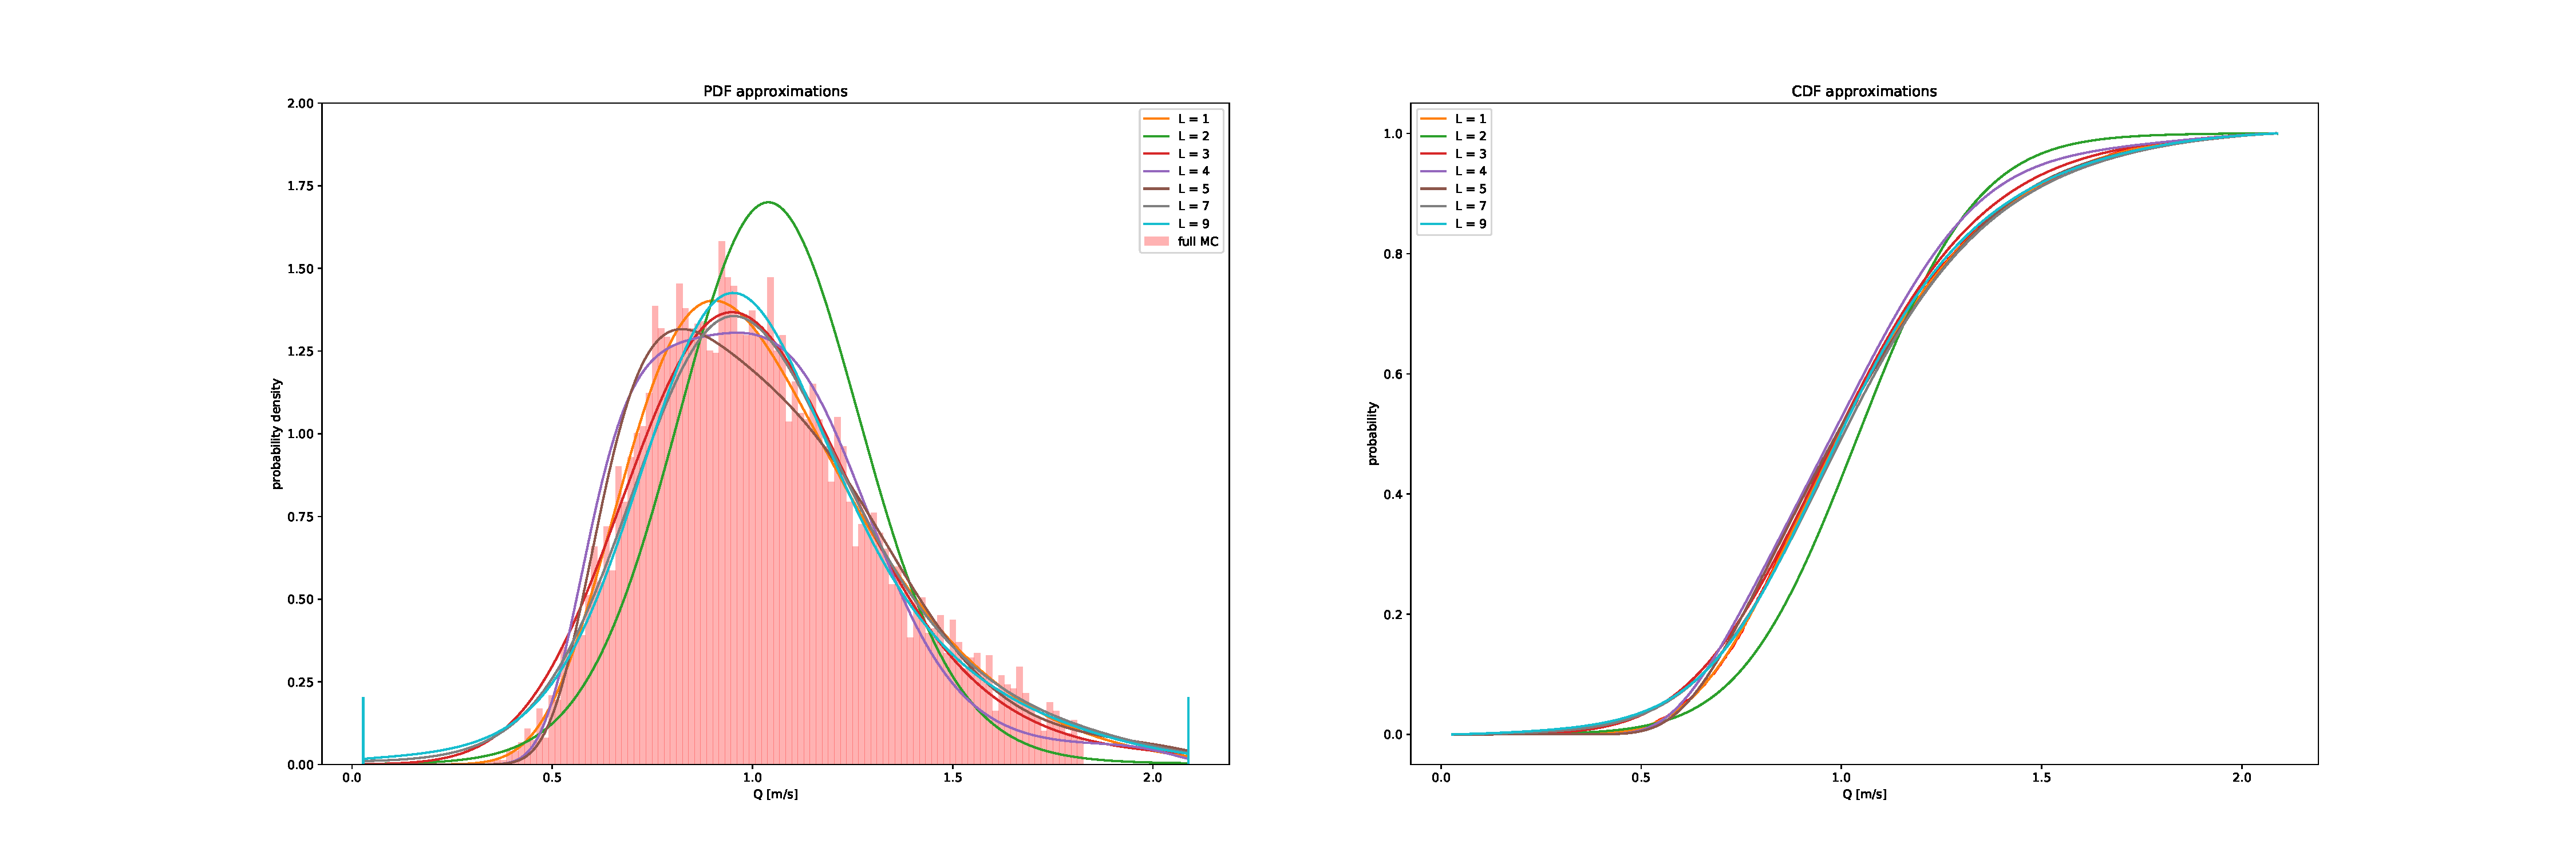
\includegraphics[width=\textwidth]{01_cond_pdf_cdf.pdf}
    \caption{Approximation a PDF of the total flux through a square domain with random conductivity. Use 11 Legendere moments.}
    \label{fig:flux_approx_pdf}
\end{figure}
\todo{Divne je, ze je ten histogram (a stejne tak vsechny histogramy prvnich urovni) uriznuty vpravo.}

\subsection{Model transport problem}
\section{Conclusions}



\bibliographystyle{plain}
\bibliography{theory.bib}








\end{document}

